%!TEX root = ../Presentation.tex

%\section*{Motivation}

\frame{
    \frametitle{Motivation}
    
    \begin{block}{\Gls{ML}}
        \tabitem Explosion in interest in \gls{ML} and \glspl{NN}\\
        \quad\tabitem Recognize objects in images\\
        \quad\tabitem Transcribe and understand spoken language\\
        \quad\tabitem Beat champions at games\\
        \tabitem Driven by compute power + availability of data\\
    \end{block}
    
    \begin{block}{\Gls{RL}}
        \tabitem Different approaches to \gls{RL}: Policy gradients and value function methods\\
        % \tabitem Sensitive to \\
        \quad\tabitem Distribution of rewards (feedback from game)\\
        \quad\tabitem Action frequency\\
        \quad\tabitem Long time horizons\\
        \quad\tabitem Backpropagation\\
        \tabitem \gls{VO} as alternative
        % \tabitem All build on simplifying assumptions and approximations\\
        % \tabitem Enables theoretical description of problems and the training of \glspl{NN} on them\\
        % \tabitem Can also introduce new problems e.g. with long time horizons\\
    \end{block}
}


\section{Introduction}

\subsection{Machine learning}


\frame{
    \frametitle{Machine learning}
    \begin{block}{What?}
        \tabitem A subset of \textbf{artificial intelligence} in the field of \textbf{computer science}\\
        \tabitem Use of \textbf{statistical techniques} to give computers the ability to \textbf{learn from data}\\
        \tabitem Goal is solving of complex tasks \textbf{without explicit programming}
    \end{block}
    
    % \begin{columns}[T]
    
    % \begin{column}{.3\textwidth}
    \begin{block}{Supervised learning}
        \tabitem Data is \textbf{labelled} in some way $\mathcal{D} = \cbra{\pa{\x_i,y_i}}_{i=1}^N$\\
        % \begin{equation}
        %     \mathcal{D} = \cbra{\pa{\x_i,y_i}}_{i=1}^N
        % \end{equation}
        \tabitem Learn mapping from $\x$ to $y$ (e.g. handwritten digit $\rightarrow$ numeric value)
    \end{block}
    % \end{column}
    
    % \begin{column}{.3\textwidth}
    \begin{block}{Unsupervised learning}
    \tabitem Data is \textbf{not labelled}: $\mathcal{D} = \cbra{\x_i}_{i=1}^N$\\
        % \begin{equation}
        %     \mathcal{D} = \cbra{\x_i}_{i=1}^N
        % \end{equation}
        \tabitem Learn underlying structure or representation of data (e.g. clustering, visualization)
    \end{block}
    
    % \end{column}
    % \begin{column}{.3\textwidth}
    \begin{block}{\Glsfirst{RL}}
        \tabitem Data is \textbf{generated} by some complex interaction with an \textbf{environment}\\
        \tabitem Learn optimal behaviour (e.g. how to play chess) based on maximizing \textbf{reward}
    \end{block}
    % \end{column}
    
    % \end{columns}
}

\subsection{Neural networks}

\frame{
    \frametitle{Neural networks}
    \begin{figure}[tbp!]
        \centering
        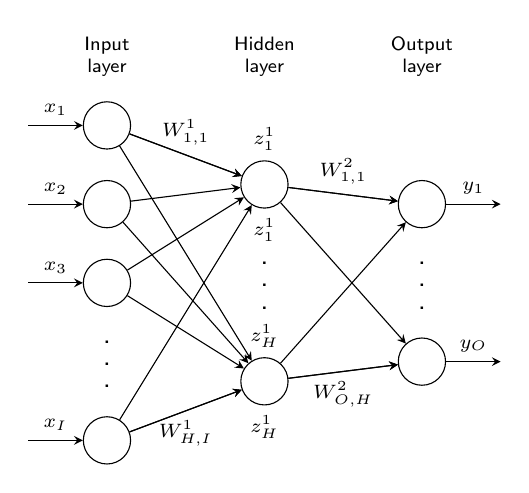
\begin{tikzpicture}[x=1.0cm, y=1.0cm, >=stealth, font=\sffamily\scriptsize]
    \tikzstyle{every neuron}=[circle, draw, minimum size=.6cm]
    \tikzstyle{neuron missing}=[draw=none, scale=2, text height=0.333cm, execute at begin node={\color{black}\tiny$\vdots$}]
    
    % Inputs nodes
    \foreach \m/\l [count=\y] in {1,2,3,missing,4}
      \node [every neuron/.try, neuron \m/.try] (input-\m) at (0,2.5-\y) {};
      
    % Hidden nodes
    \foreach \m [count=\y] in {1,missing,2} {
        \node [every neuron/.try, neuron \m/.try ] (hidden-\m) at (2,2-\y*1.25) {};
    }
        % \ifthenelse{\y=2}
        %     {\node [every neuron/.try, neuron \m/.try ] (hidden-\m) at (2,2-\y*1.25) {};}
        %     {\node [every neuron/.try, neuron \m/.try ] (hidden-\m) at (2,2-\y*1.25) {$a_\m^\bra{0}$};}
        % }
      %\node [every neuron/.try, neuron \m/.try ] (hidden-\m) at (2,2-\y*1.25) {$a_\m^\bra{0}$};
      
    % Outputs nodes
    \foreach \m [count=\y] in {1,missing,2}
      \node [every neuron/.try, neuron \m/.try ] (output-\m) at (4,1.5-\y) {};
      
    % Names on inputs
    \foreach \l [count=\i] in {1,2,3,I}
      \draw [<-] (input-\i) -- ++(-1,0)
        node [above, midway] {$x_\l$};
        
    % Names on hidden
    \foreach \l [count=\i] in {1,H} {
        \ifthenelse{\i=1}
            {\node [above] at (hidden-\i.north) {$z^\bra{1}_\l$};}
            {\node [below] at (hidden-\i.south) {$z^\bra{1}_\l$};}
    }
      
    % Names on outputs
    \foreach \l [count=\i] in {1,O}
      \draw [->] (output-\i) -- ++(1,0)
        node [above, midway] {$y_\l$};
        
    % Inputs -> Hidden
    \foreach \i in {1,...,4} {
      \foreach \j in {1,...,2} {
        %\draw [->] (input-\i) -- (hidden-\j);
        \ifthenelse{\i=1 \AND \j=1 \OR \i=4 \AND \j=2}
            {}
            {\draw [->] (input-\i) -- (hidden-\j);}
        }
    }
    \draw [->] (input-1) --node[above]{$W^{\bra{1}}_{1,1}$} (hidden-1);
    \draw [->] (input-4) --node[below]{$W^{\bra{1}}_{H,I}$} (hidden-2);
        
    % Hidden -> Outputs
    \foreach \i in {1,...,2}  {
      \foreach \j in {1,...,2} {
        % \draw [->] (hidden-\i) -- (output-\j);
        \ifthenelse{\i=1 \AND \j=1 \OR \i=2 \AND \j=2}
            {}
            {\draw [->] (hidden-\i) -- (output-\j);}
        }
    }
    \draw [->] (hidden-1) --node[above]{$W^{\bra{2}}_{1,1}$} (output-1);
    \draw [->] (hidden-2) --node[below]{$W^{\bra{2}}_{O,H}$} (output-2);
    
    % Layer names
    \foreach \l [count=\x from 0] in {Input, Hidden, Output}
      \node [align=center, above] at (\x*2,2) {\l \\ layer};
\end{tikzpicture}
        \caption{\Gls{FNN} with a single hidden layer and an output layer.}
        \label{fig: Neural networks: multilayer perceptron (FNN)}
    \end{figure}
}

% \frame{
%     \frametitle{Neural networks}
%     \begin{figure}[tbp!]
%         \begin{subfigure}[b]{0.40\textwidth}
%             \centering
%             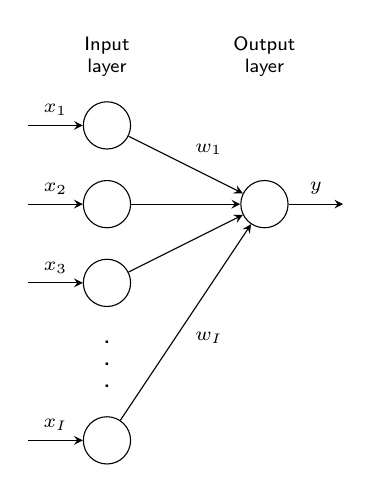
\begin{tikzpicture}[x=1.0cm, y=1.0cm, >=stealth, font=\sffamily\scriptsize]
    \tikzstyle{every neuron}=[circle, draw, minimum size=.6cm]
    \tikzstyle{neuron missing}=[draw=none, scale=2, text height=0.333cm, execute at begin node={\color{black}\tiny$\vdots$}]
    
    % Input nodes
    \foreach \m/\l [count=\y] in {1,2,3,missing,4}
        \node [every neuron/.try, neuron \m/.try] (input-\m) at (0,2.5-\y) {};
      
    % Output node
    \node [every neuron/.try, neuron 1/.try ] (output-1) at (2,1.5-1) {};

    % Names on input arrows
    \foreach \l [count=\i] in {1,2,3,I}
        \draw [<-] (input-\i) -- ++(-1,0) node [above, midway] {$x_\l$};
    
    % Name on output arrow
    \draw [->] (output-1) -- ++(1,0) node [above, midway] {$y$};
    
    % Inputs -> Outputs
    \draw [->] (input-1) -- node[above right]{$w_{1}$} (output-1);
    \draw [->] (input-2) -- (output-1);
    \draw [->] (input-3) -- (output-1);
    \draw [->] (input-4) -- node[below right]{$w_{I}$} (output-1);
    
    % Layer names
    \foreach \l [count=\x from 0] in {Input\\layer, Output\\layer}
        \node [align=center, above] at (\x*2,2) {\l};
\end{tikzpicture}
%             \caption{}
%             \label{fig: Neural networks: Perceptron}
%         \end{subfigure}
%         \hfill
%         \begin{subfigure}[b]{0.58\textwidth}
%             \centering
%             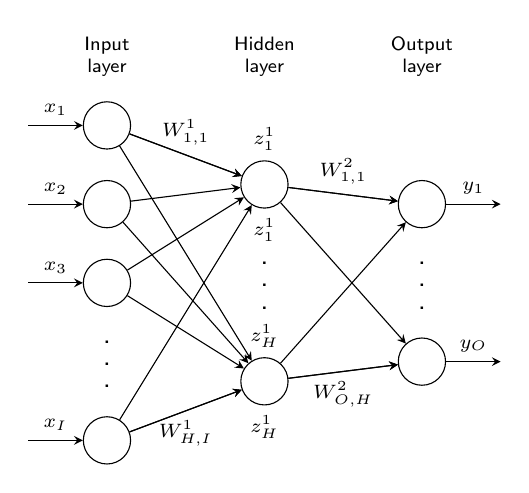
\begin{tikzpicture}[x=1.0cm, y=1.0cm, >=stealth, font=\sffamily\scriptsize]
    \tikzstyle{every neuron}=[circle, draw, minimum size=.6cm]
    \tikzstyle{neuron missing}=[draw=none, scale=2, text height=0.333cm, execute at begin node={\color{black}\tiny$\vdots$}]
    
    % Inputs nodes
    \foreach \m/\l [count=\y] in {1,2,3,missing,4}
      \node [every neuron/.try, neuron \m/.try] (input-\m) at (0,2.5-\y) {};
      
    % Hidden nodes
    \foreach \m [count=\y] in {1,missing,2} {
        \node [every neuron/.try, neuron \m/.try ] (hidden-\m) at (2,2-\y*1.25) {};
    }
        % \ifthenelse{\y=2}
        %     {\node [every neuron/.try, neuron \m/.try ] (hidden-\m) at (2,2-\y*1.25) {};}
        %     {\node [every neuron/.try, neuron \m/.try ] (hidden-\m) at (2,2-\y*1.25) {$a_\m^\bra{0}$};}
        % }
      %\node [every neuron/.try, neuron \m/.try ] (hidden-\m) at (2,2-\y*1.25) {$a_\m^\bra{0}$};
      
    % Outputs nodes
    \foreach \m [count=\y] in {1,missing,2}
      \node [every neuron/.try, neuron \m/.try ] (output-\m) at (4,1.5-\y) {};
      
    % Names on inputs
    \foreach \l [count=\i] in {1,2,3,I}
      \draw [<-] (input-\i) -- ++(-1,0)
        node [above, midway] {$x_\l$};
        
    % Names on hidden
    \foreach \l [count=\i] in {1,H} {
        \ifthenelse{\i=1}
            {\node [above] at (hidden-\i.north) {$z^\bra{1}_\l$};}
            {\node [below] at (hidden-\i.south) {$z^\bra{1}_\l$};}
    }
      
    % Names on outputs
    \foreach \l [count=\i] in {1,O}
      \draw [->] (output-\i) -- ++(1,0)
        node [above, midway] {$y_\l$};
        
    % Inputs -> Hidden
    \foreach \i in {1,...,4} {
      \foreach \j in {1,...,2} {
        %\draw [->] (input-\i) -- (hidden-\j);
        \ifthenelse{\i=1 \AND \j=1 \OR \i=4 \AND \j=2}
            {}
            {\draw [->] (input-\i) -- (hidden-\j);}
        }
    }
    \draw [->] (input-1) --node[above]{$W^{\bra{1}}_{1,1}$} (hidden-1);
    \draw [->] (input-4) --node[below]{$W^{\bra{1}}_{H,I}$} (hidden-2);
        
    % Hidden -> Outputs
    \foreach \i in {1,...,2}  {
      \foreach \j in {1,...,2} {
        % \draw [->] (hidden-\i) -- (output-\j);
        \ifthenelse{\i=1 \AND \j=1 \OR \i=2 \AND \j=2}
            {}
            {\draw [->] (hidden-\i) -- (output-\j);}
        }
    }
    \draw [->] (hidden-1) --node[above]{$W^{\bra{2}}_{1,1}$} (output-1);
    \draw [->] (hidden-2) --node[below]{$W^{\bra{2}}_{O,H}$} (output-2);
    
    % Layer names
    \foreach \l [count=\x from 0] in {Input, Hidden, Output}
      \node [align=center, above] at (\x*2,2) {\l \\ layer};
\end{tikzpicture}
%             \caption{}
%             \label{fig: Neural networks: MLP}
%         \end{subfigure}
%         \caption{\subref{fig: Neural networks: Perceptron} Perceptron model due to Rosenblatt \cite{Rosenblatt1957}. The single scalar output is computed as the sign of the weighted sum of inputs. \subref{fig: Neural networks: MLP} \Gls{FNN} with a single hidden layer and an output layer.}
%         \label{fig: Neural networks: Single and multilayer perceptron (FNN)}
%     \end{figure}
% }

\frame{
    \frametitle{Neural networks}
    \begin{block}{Why?}
        \tabitem Huge flexibility and representational power\\
        \tabitem Can learn \textbf{representations and mappings} from raw data
    \end{block}
    \begin{block}{How?}
        \begin{enumerate}
            \item Forward pass: Evaluation of network on task and calculation of error, $f(\x,\w)$\\
            \item Backward pass: Change of parameters/weights in direction that reduces error\\
        \end{enumerate}
    \end{block}
    \begin{block}{Backpropagation}
        \begin{equation}\label{eq: Neural networks: Backpropagation in FNN to arbitrary depth hidden unit}
            \pderiv{f_i}{\W^\bra{l}} =  \underbrace{
                \pderiv{E}{\a^\bra{L}}\pderiv{\a^\bra{L}}{\z^\bra{L}}
                \pderiv{\z^\bra{L}}{\a^\bra{L-1}}\pderiv{\a^\bra{L-1]}}{\z^\bra{L-1}}
                \dots
                \pderiv{\z^\bra{l+1}}{\a^\bra{l}} \pderiv{\a^\bra{l}}{\z^\bra{l}}
            }_{\deltab^\bra{l}} \pderiv{\z^\bra{l}}{\W^\bra{l}}
        % \pderiv{f_i}{\z^\bra{l}} = 
        % \underbrace{
        %     \underbrace{
        %         \underbrace{
        %             \pderiv{f_i}{\a^\bra{L}}\pderiv{\a^\bra{L}}{\z^\bra{L}}
        %         }_{\deltab^\bra{L}}
        %         \pderiv{\z^\bra{L}}{\a^\bra{L-1}}\pderiv{\a^\bra{L-1]}}{\z^\bra{L-1}}
        %     }_{\deltab^\bra{L-1}}
        %     \dots
        %     \pderiv{\z^\bra{l+1}}{\a^\bra{l}} \pderiv{\a^\bra{l}}{\z^\bra{l}}
        % }_{\deltab^\bra{l}}
    \end{equation}
    \end{block}
}


\frame{
    \frametitle{Neural networks}
    \begin{block}{But!}
        \tabitem Backpropagation requires differentiable architecture\\
        \tabitem If \textbf{nondifferentiability} is introduced, backpropagation does not work without modification or tricks\\
        \quad\tabitem Nondifferentiable network (discrete latent variables, stochastic elements)\\
        \quad\tabitem Nondifferentiable error (e.g. discrete actions/rewards as in \gls{RL})\\
    \end{block}
    \begin{block}{This work}
        \tabitem How can gradients be estimated when the error (or network) is nondifferentiable?\\
    \end{block}
}


\subsection{Evolution strategies}

\frame{
    \frametitle{Evolution strategies}
    % \begin{block}{Notation}
    %     \begin{itemize}
    %         \item Let $\y$ be the result of forward propagating input $\x$ in a network with weights $\w$.\\
    %         % \item The loss is then $f(\y,\w)$ or $f(\w)$, letting the input be implicit.\\
    %         \item Let $f(\y,\w)$ or simply $f(\w)$ be some loss or objective function computed on $\y$.\\
    %     \end{itemize}
    % \end{block}
    \begin{block}{Stochastic estimation of neural network gradient}
        \tabitem Taylor series gives a gradient estimate for any objective/error $f$ dependent on parameters $\w$.\\
        \tabitem With $\epsilonb\sim\mathcal{N}(\0,\I)$
        \begin{align}\label{eq: Theory: Taylor: Multivariate Taylor expansion}
            f(\w+\epsilonb) &\approx f(\w) + \epsilonb\transpose \nabla_\w f(\w) + \frac{1}{2}\epsilonb\transpose\H(\w)\epsilonb\\
        % \shortintertext{Multiply by $\epsilonb$ and take expectation}
            \text{E}\left[f(\w+\epsilonb)\epsilonb\right] &\approx \text{E}\left[\epsilonb\epsilonb\transpose\right]\nabla_\w\ f(\w) = \nabla_\w f(\w)\nonumber
        \end{align}
        \tabitem With isotropic perturbation variance $\sigma^2$, the gradient estimator becomes
        \begin{equation}
            \nabla_\w f(\w) \approx \sigma^{-1}\text{E}\left[ f(\w+\sigma\epsilonb)\epsilonb\right] \approx \frac{1}{N\sigma}\sum_{n=1}^N f(\w+\sigma\epsilonb_n)\epsilonb_n
        \end{equation}
        \tabitem As in OpenAI's recent article \cite{Salimans2017} on \glspl{ES}.
    \end{block}
}

\frame{
    \frametitle{Evolution strategies}
    \begin{algorithm}[H]
        \footnotesize{
    	\caption{Parallelized evolution strategy \label{alg: Evolution strategy}}
    	}
        \footnotesize{
    	\begin{algorithmic}[1]
    		\Require{Objective function $f(\x)$, learning rate $\eta$, perturbation variance $\sigma$}
    		\Initialize{$N$ workers with known random seeds}
    		\Repeat
    			\For{each \gls{CPU} $i=1,\dots,N$} \Comment{Parallelized}
    			    \State Draw random seed $s_i$
    				\State Sample $\epsilonb_i\sim \mathcal{N}(\0,\I)$
    				\State Evaluate fitness $f(\w+\sigma\epsilonb_i)$
    			\EndFor
    			\State Share $N$ scalar fitnesses, $f(\w+\sigma\epsilonb_i)$ and seeds, $s_i$, between all \glspl{CPU}.
    			\For{each worker $i=1,\dots,N$} \Comment{Parallelized}
    				\State Reconstruct all perturbations $\epsilonb_j$ for $j=1,\dots,N$ using known random seeds.
    				\State Compute gradient
    				$$\nabla_\w f(\w) \approx \frac{1}{N\sigma}\sum_{n=1}^N f(\w+\sigma\epsilonb_n)\epsilonb_n$$
    				\State Update parameters $\w \gets \w - \eta\nabla_\w f(\w)$
    			\EndFor
    		\Until{stopping criteria met}
    	\end{algorithmic}
    	}
    \end{algorithm}
}



\frame{
    \frametitle{Himmelblau example (\#1)}
    \begin{figure}[tbp!]
        \begin{subfigure}[b]{0.49\textwidth}
            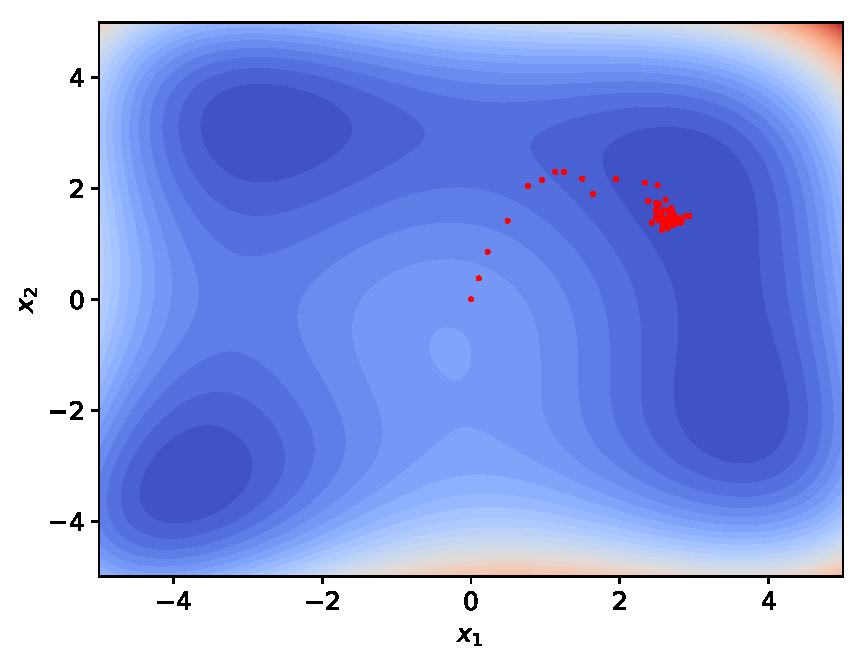
\includegraphics[width=\textwidth]{graphics/var-opt-conv/ES-himmelblau-convergence.pdf}
            \caption{}
            \label{fig: Theory: var-opt-conv-ES-himmelblau-convergence}
        \end{subfigure}
        \hfill
        \begin{subfigure}[b]{0.49\textwidth}
            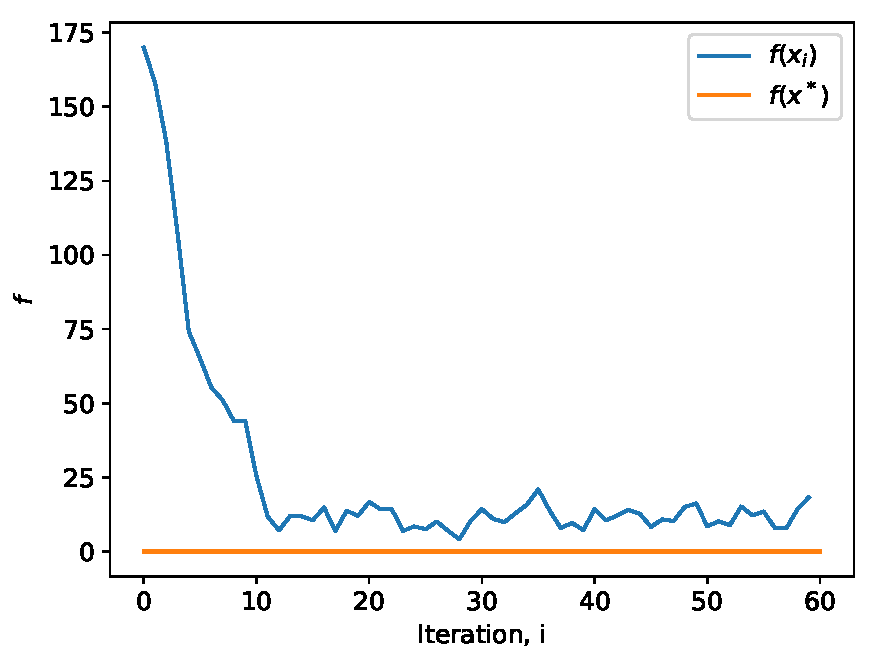
\includegraphics[width=\textwidth]{graphics/var-opt-conv/ES-himmelblau-f.pdf}
            \caption{}
            \label{fig: Theory: var-opt-conv-ES-himmelblau-f}
        \end{subfigure}
        \caption{\subref{fig: Theory: var-opt-conv-ES-himmelblau-convergence} Convergence of the evolutionary strategy used by \cite{Salimans2017}. \subref{fig: Theory: var-opt-conv-ES-himmelblau-f} Objective function value at each iteration of the algorithm. The algorithm finds a minimum but struggles to converge due to the fixed search distribution variance.}
        \label{fig: Theory: var-opt-conv-ES-himmelblau}
    \end{figure}
}

\frame{
    \frametitle{Evolution strategies}

    \begin{block}{Gradient variance}
        \tabitem The variance of the gradient estimator is
        \begin{equation}\label{eq: Gradient variance: ES Isoptropic Gaussian in terms of f and eps}
            \text{Var}\left[\nabla_\w f(\w)\right]
            \approx \text{Var}\left[\frac{1}{N\sigma}\sum_{n=1}^N f(\w+\sigma\epsilonb_n)\epsilonb_n\right]
            = \frac{1}{N\sigma^2}\text{Var}\bra{f(\w+\sigma\epsilonb)\epsilonb} \ . 
        \end{equation}
        \tabitem In univariate case, for small $\epsilon$ or $\sigma$, $f(w+\sigma\epsilon) \approx f(w) + \sigma\epsilon f'(w)$ and
        \begin{align}
            \text{Var}\left[f'(w)\right]
            &\approx \frac{1}{N\sigma^2}\text{Var}\bra{f(w)\epsilon + \sigma\epsilon^2 f'(w)} \nonumber\\
            &= \frac{1}{N\sigma^2}\pa{f(w)^2 + 2f'(w)^2\sigma^2}\nonumber\\
            &= \frac{1}{N\sigma^2}f(w)^2 + \frac{2}{N}f'(w)^2
        \end{align}
        % \tabitem By Taylor expansion for small $\epsilonb$ or $\sigma$, $f(\w+\sigma\epsilonb) \approx f(\w) + \sigma\epsilonb\transpose\nabla_\w f(\w)$ and
        % \begin{align}
        %     \text{Var}\left[\nabla_\w f(\w)\right]
        %     &\approx \frac{1}{N\sigma^2}\text{Var}\bra{f(\w)\epsilonb + \sigma\epsilonb\epsilonb\transpose \nabla_\w f(\w)} \nonumber\\
        %     &= \frac{1}{N\sigma^2}\pa{f(\w)^2\I + \sigma^2(d+1)\nabla_\w f(\w)\nabla_\w f(\w)\transpose}\nonumber\\
        %     &= \frac{1}{N\sigma^2}f(\w)^2 + \frac{d+1}{N}\nabla_\w f(\w)\nabla_\w f(\w)\transpose
        % \end{align}
        % \tabitem For $\sigma\rightarrow0$, the variance of the gradient estimate explodes.
    \end{block}
    \begin{block}{Summary}
        \tabitem Variance of gradient explodes as $\sigma\rightarrow0$\\
        \tabitem $\sigma$ must go to zero to precisely locate minima, but how?\\
    \end{block}
}


\section{Variational optimization}

\subsection{Definition}

\frame{
    \frametitle{Formulation}
    \begin{block}{Variational upper bound}
        \tabitem \Gls{VO} provides a more rigorous framework for evolutionary strategies \cite{Staines2012}.\\
        \begin{equation}\label{eq: Theory: Variational optimization variational upper bound}
            f(\w^*) = \min_{\w} f(\w) \leq \text{E}\bra{f(\w)}_{p(\w|{\thetab})} \equiv U({\thetab})
        \end{equation}
        \tabitem Minimize the variational upper bound $\min_\thetab U(\thetab)$ rather than $f(\w)$
    \end{block}
    \begin{block}{Gradient of upper bound}
        \tabitem The \gls{VO} upper bound is differentiable using the log-derivative trick
        \begin{align}
        \nabla_{\thetab} U({\thetab}) 
        &= \nabla_{\thetab} \text{E}\bra{f(\w)}_{p(\w|\thetab)}\nonumber\\
        &= \nabla_{\thetab}\int f(\w)p(\w|{\thetab}) \text{d}\w\nonumber\\
        &= \int f(\w) p(\w|{\thetab})\nabla_{\thetab}\log p(\w|{\thetab}) \text{d}\w\nonumber\\
        &= \text{E}\bra{f(\w)\nabla_{\thetab}\log p(\w|{\thetab})}_{p(\w|{\thetab})}\label{eq: Theory: Variational optimization gradient estimator general search distribution}
        \end{align}
    \end{block}
}


% \subsection{Algorithm}

\frame{
    \frametitle{Formulation}
    \begin{algorithm}[H]
        \footnotesize{
    	\caption{Parallelized \glsfirst{VO}. Adapted from \cite{Wierstra2008} \label{alg: Canonical variational optimization}}
    	}
        \footnotesize{
    	\begin{algorithmic}[1]
    		\Require{Objective function $f(\x)$, learning rate $\eta$, {\color{dtured} search distribution $p(\w|\thetab)$}}
    		\Initialize{$N$ workers with known random seeds}
    		\Repeat
    			\For{each \gls{CPU} $i=1,\dots,N$} \Comment{Parallelized}
    			    \State Draw random seed $s_i$
    				\State {\color{dtured} Sample $\w_i\sim p(\w|\thetab)$}
    				\State Evaluate fitness $f(\w_i)$
    			\EndFor
    			\State Share $N$ scalar fitnesses, $f(\w_i)$ and seeds, $s_i$, between all \glspl{CPU}.
    			\For{each worker $i=1,\dots,N$} \Comment{Parallelized}
    				\State Reconstruct all perturbations $\w_j$ for $j=1,\dots,N$ using known random seeds.
    				\State {\color{dtured} Compute search distribution and upper bound gradient}
    				{\color{dtured} $$\nabla_\thetab U(\thetab) = \frac{1}{N}\sum_{n=1}^N f(\w_i) \nabla_\thetab\log p(\w_i|\thetab)$$}
    				\State {\color{dtured} Update search distribution parameters $\thetab \gets \thetab - \eta\nabla_\thetab U(\thetab)$ }
    			\EndFor
    		\Until{stopping criteria met}
    	\end{algorithmic}
    	}
    \end{algorithm}
}


\frame{
    \frametitle{Augmentations}
    \begin{block}{Network}
        \tabitem Any architecture (dense, convolutional, recurrent)\\
        \tabitem Any training improvement technique (batch normalization, dropout, initialization)\\
    \end{block}
    \begin{block}{Optimizer}
        \tabitem Any optimizer can be used on the gradients\\
        \tabitem Optimizing in $d\gg N$ regime, always moving in subspace of network weight space\\
        \tabitem Momentum works by reducing variance and remembering good subspace
    \end{block}
    \begin{block}{\gls{VO} algorithm}
        \tabitem Natural gradient\\
        \tabitem Variance reduction\\
            \quad\tabitem Antithetic sampling\\
            \quad\tabitem Local reparameterization\\
        \tabitem Other\\
            \quad\tabitem Rescaling of perturbations by sensitivities\\
            \quad\tabitem Importance mixing\\
            \quad\tabitem Adaptation sampling
    \end{block}
}



\subsection{Search distributions}

\frame{
    \frametitle{Search distributions}
    \begin{block}{Univariate Gaussian}
        \begin{equation}
            p(w|\thetab) = \mathcal{N}\pa{w|\mu,\sigma^2} = \frac{1}{\sqrt{2\pi\sigma^2}}\exp\pa{-\frac{1}{2\sigma^2}\pa{w-\mu}^2}
        \end{equation}
        \tabitem Take log and derivatives w.r.t. $\mu$ and $\sigma$ with $\epsilon\sim\mathcal{N}\pa{0,1}$,
        % \begin{equation}
        %     \log\mathcal{N}\pa{w\middle\mu,\sigma^2} = -\frac{1}{2}\log2\pi - \frac{1}{2}\log\sigma^2 - \frac{1}{2\sigma^2}\pa{w-\mu}^2
        % \end{equation}
        \begin{equation}
            \begin{aligned}
                \pderiv{}{\mu}\log\mathcal{N}(w|\mu,\sigma^2) &= \frac{1}{\sigma^2}(w-\mu) = \frac{1}{\sigma}\epsilon\\
                \pderiv{}{\sigma^2}\log\mathcal{N}(w|\mu,\sigma^2) &= -\frac{1}{2\sigma^2} + \frac{1}{4\sigma^4}(w-\mu)^2  = \frac{1}{\sigma^2}\pa{\epsilon^2-1}. % = \frac{1}{2\sigma^2}\left(\frac{1}{\sigma^2}(x-\mu)^2 - 1\right).
            \end{aligned}\label{eq: Theory: Variational optimization univariate gaussian search gradients}
        \end{equation}
        \tabitem Use \eqref{eq: Theory: Variational optimization gradient estimator general search distribution} to obtain the univariate Gaussian search gradient
        \begin{align}\label{eq: Theory: Variational optimization univariate gaussian gradient estimators}
            \pderiv{}{\mu}U(\mu,\sigma^2) &= \frac{1}{\sigma}\text{E}\bra{f(\mu + \sigma\epsilon)\epsilon} \approx \frac{1}{N\sigma}\sum_{n=1}^N f(\mu+\sigma\epsilon_n)\epsilon_n\\
            \pderiv{}{\sigma^2}U(\mu,\sigma^2) &= \frac{1}{2\sigma^2}\text{E}\bra{f(\mu + \sigma\epsilon)\left(\epsilon^2-1\right)} \approx \frac{1}{2N\sigma^2}\sum_{n=1}^N f(\mu + \sigma\epsilon_n)\left(\epsilon_n^2-1\right)\nonumber
        \end{align}
        % \tabitem This is the univariate case of the estimator of \cite{Salimans2017} but now with way to vary $\sigma$.
    \end{block}
}

\frame{
    \frametitle{Nondifferentiable objective}
    \begin{figure}[tbp!]
        \begin{subfigure}[b]{0.49\textwidth}
            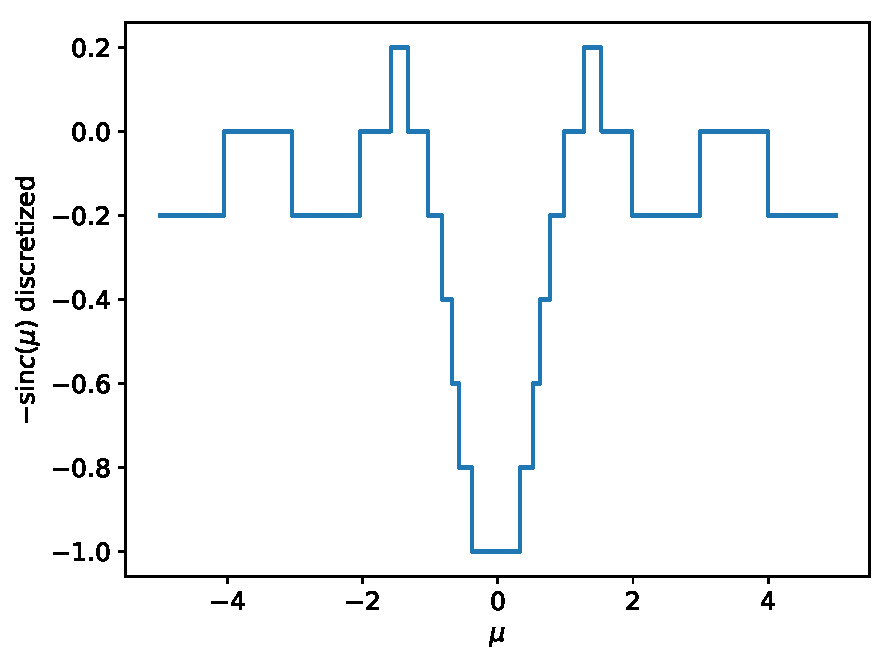
\includegraphics[width=\textwidth]{graphics/var-opt-intu/variational-optimization-function-sinc_quantized.pdf}
            \caption{}
            \label{fig: Theory: var-opt-intu-sinc-quantized-function}
        \end{subfigure}
        \hfill
        \begin{subfigure}[b]{0.49\textwidth}
            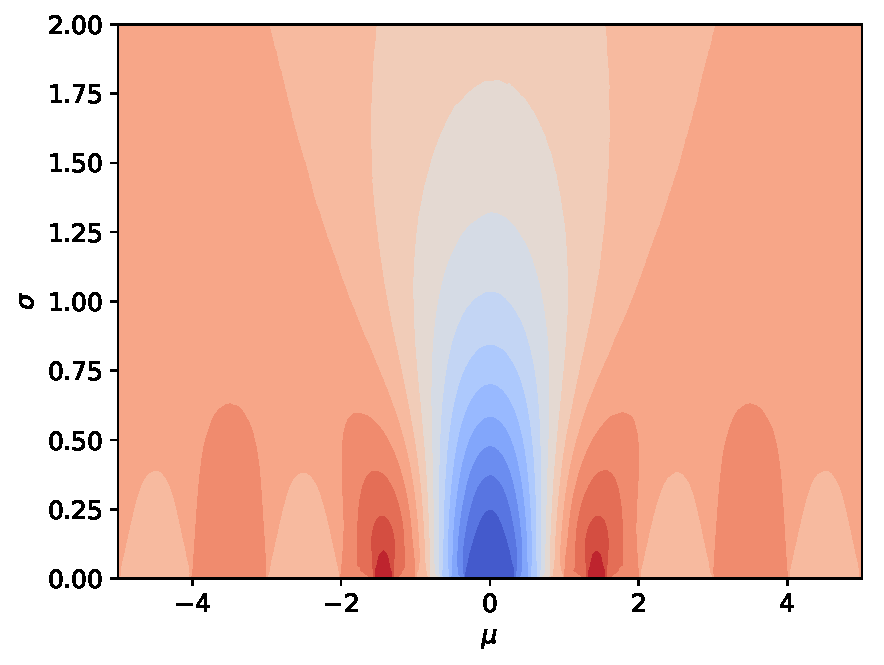
\includegraphics[width=\textwidth]{graphics/var-opt-intu/variational-optimization-contour-sinc_quantized.pdf}
            \caption{}
            \label{fig: Theory: var-opt-intu-sinc-quantized-contour}
        \end{subfigure}
        \caption{Using a univariate Gaussian search distribution, the 1-dimensional discretized and nondifferentiable $\sinc$ function is turned into a 2-dimensional differentiable variational upper bound. The \gls{VO} upper bound tends to nondifferentiability for $\sigma\rightarrow0$. Figures inspired by \cite{Huszar2017}.}
        \label{fig: Theory: var-opt-intu-sinc-quantized}
    \end{figure}
}

\frame{
    \frametitle{Shallow and narrow minima}
    \begin{figure}[tbp!]
        \begin{subfigure}[b]{0.49\textwidth}
            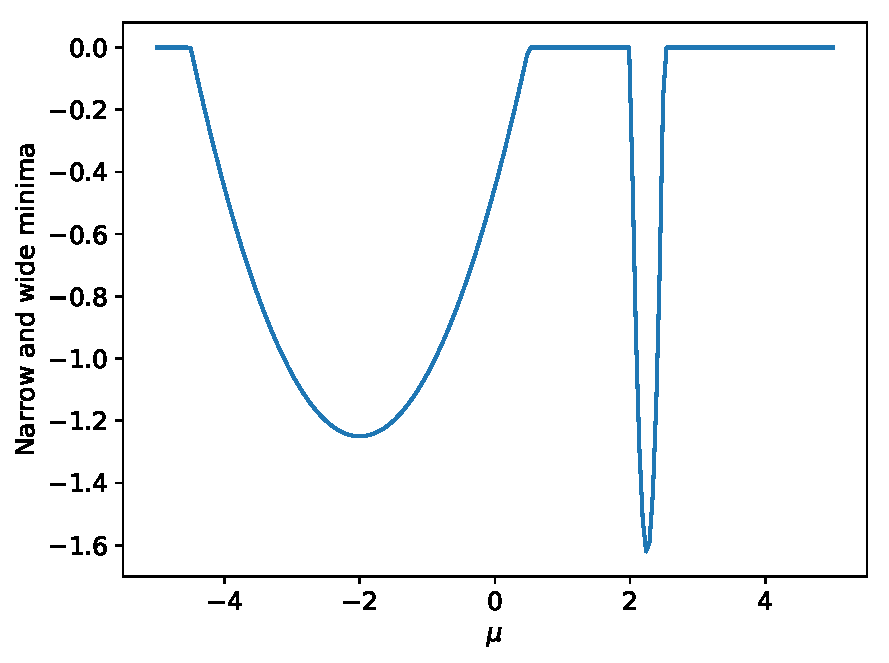
\includegraphics[width=\textwidth]{graphics/var-opt-intu/variational-optimization-function-narrow_vs_wide.pdf}
            \caption{}
            \label{fig: Theory: var-opt-intu-narrow-vs-wide-function}
        \end{subfigure}
        \hfill
        \begin{subfigure}[b]{0.49\textwidth}
            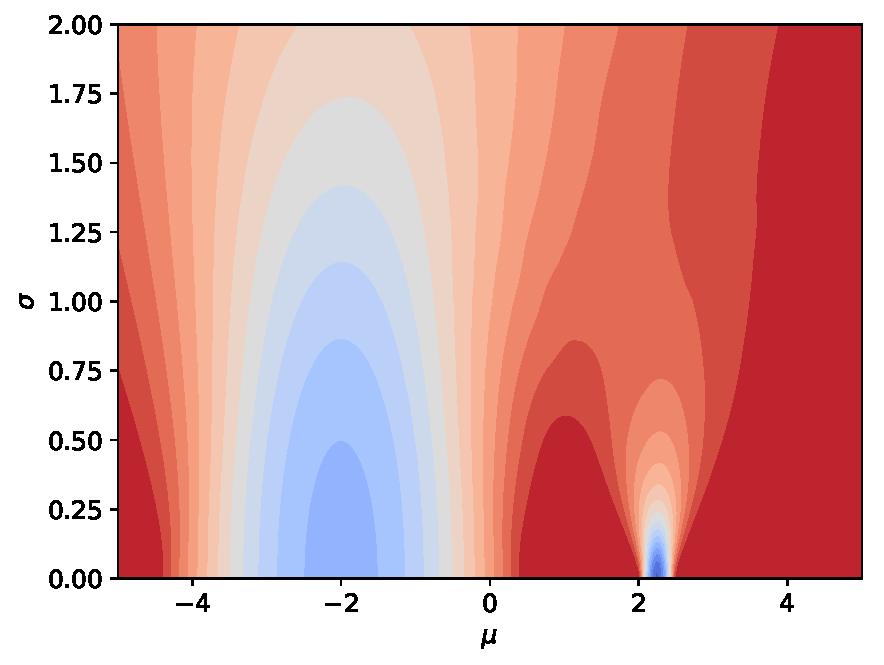
\includegraphics[width=\textwidth]{graphics/var-opt-intu/variational-optimization-contour-narrow_vs_wide.pdf}
            \caption{}
            \label{fig: Theory: var-opt-intu-narrow-vs-wide-contour}
        \end{subfigure}
        \caption{\subref{fig: Theory: var-opt-intu-narrow-vs-wide-function} A function with a low curvature local minimum and a high curvature global minimum. \subref{fig: Theory: var-opt-intu-narrow-vs-wide-contour} The contours of the corresponding Gaussian \gls{VO} objective. This illustrates the tendency of \gls{VO} to prefer low curvature minima over high curvature minima if situated near each other. Figures inspired by \cite{Huszar2017}.}
        \label{fig: Theory: var-opt-intu-narrow-vs-wide}
    \end{figure}
}

\frame{
    \frametitle{Search distributions}
    \begin{block}{Isotropic Gaussian}
        \tabitem Let $\Sigmab = \sigma^2\I$. Then
        \begin{align}
            \nabla_\mub U(\mub,\sigma^2) &\approx \frac{1}{N\sigma}\sum_{n=1}^N f(\mub+\sigma\epsilonb_n)\epsilonb_n\\
            \nabla_{\sigmab^2} U(\mub,\sigma^2) &\approx \frac{1}{2N\sigma^2}\sum_{n=1}^N f(\mub + \sigma\epsilonb_n)\left(\epsilonb_n^2-d\right)\nonumber
        \end{align}
    \end{block}
    \begin{block}{Separable Gaussian}
        \tabitem Let $\sigmab^2 = \bmat{\sigma_1^2 & \sigma_2^2 & \cdots & \sigma_d^2}\transpose$ and $\Sigmab = \text{diag}\pa{\sigmab^2}$. Then
        \begin{align}
            \nabla_\mub U(\mub,\sigmab^2) &\approx \frac{\sigmab^{-1}}{N}\odot\sum_{n=1}^N f(\mub+\sigmab\odot\epsilonb_n)\epsilonb_n\\
            \nabla_{\sigmab^2} U(\mub,\sigmab^2) &\approx \frac{\sigmab^{-2}}{2N}\odot\sum_{n=1}^N f(\mub + \sigmab\odot\epsilonb_n)\pa{\epsilonb^2 - 1}\nonumber
        \end{align}
    \end{block}
}

% \frame{
%     \frametitle{Search distributions}
%     \begin{block}{Isotropic Gaussian}
%         \tabitem Let $\Sigmab = \sigma^2\I$ then
%         \begin{equation}
%             \begin{aligned}
%                 \nabla_\mub \log\mathcal{N}(\w|\mub,\sigma^2\I) &= \frac{1}{\sigma^2}(\w-\mub) = \frac{1}{\sigma}\epsilonb\\
%                 \nabla_{\sigma^2} \log\mathcal{N}(\w|\mub,\sigma^2\I) &= -\frac{d}{2\sigma^2} + \frac{1}{2\sigma^4}(\w-\mub)\transpose(\w-\mub) = \frac{1}{2\sigma^2}\left(\epsilonb\transpose\epsilonb - d\right)
%             \end{aligned}
%         \end{equation}
%         \tabitem Isotropic Gaussian search gradient
%         \begin{align}
%             \nabla_\mub U(\mub,\sigma^2) &= \frac{1}{\sigma}\text{E}\bra{f(\mub + \sigma\epsilonb)\epsilonb} \approx \frac{1}{N\sigma}\sum_{n=1}^N f(\mub+\sigma\epsilonb_n)\epsilonb_n\\
%             \nabla_{\sigmab^2} U(\mub,\sigma^2) &= \frac{1}{2\sigma^2}\text{E}\bra{f(\mub + \sigma\epsilonb)\left(\epsilonb\transpose\epsilonb-d\right)} \approx \frac{1}{2N\sigma^2}\sum_{n=1}^N f(\mub + \sigma\epsilonb_n)\left(\epsilonb_n^2-d\right)\nonumber
%         \end{align}
%         \tabitem Identical to the estimator of \cite{Salimans2017}, again with method for adapting $\sigma$.
%     \end{block}
% }

% \frame{
%     \frametitle{Search distributions}
%     \begin{block}{Separable Gaussian}
%         \tabitem Let $\sigmab^2 = \bmat{\sigma_1^2 & \sigma_2^2 & \cdots & \sigma_d^2}\transpose$ so $\Sigmab = \pa{\sigmab^2\e\transpose}\odot\I$ and
%         \begin{align}
%             \log\mathcal{N}\pa{\w|\mub, (\sigmab^2\e\transpose)\odot\I} &= -\frac{d}{2}\log(2\pi) - \frac{1}{2}\e\transpose\log\pa{\sigmab^2} - \frac{1}{2}\pa{\sigmab^{-2}}\transpose(\w-\mub)^2\nonumber\\
%             \nabla_\mub \log\mathcal{N}(\w|\mub,(\sigmab^2\e\transpose)\odot\I) &= \sigmab^{-2} \odot (\w-\mub) = \sigmab^{-1} \odot \epsilonb\\
%             \nabla_{\sigmab^2} \log\mathcal{N}(\w|\mub,(\sigmab^2\e\transpose)\odot\I) &= -\frac{1}{2}\sigmab^{-2} + \frac{1}{2} \sigmab^{-4}\odot(\w-\mub)^2 = -\frac{1}{2}\sigmab^{-2} \odot \pa{\epsilonb^2 - 1}\nonumber
%         \end{align}
%         \tabitem Separable Gaussian search gradient
%         \begin{align}
%             \nabla_\mub U(\mub,\sigma^2) &= \sigmab^{-1}\odot\text{E}\bra{f(\mub + \sigmab\odot\epsilonb)\epsilonb} \approx \sigmab^{-1}\odot\frac{1}{N}\sum_{n=1}^N f(\mub+\sigmab\odot\epsilonb_n)\epsilonb_n\nonumber\\
%             \nabla_{\sigmab^2} U(\mub,\sigma^2) &= \frac{1}{2}\odot\text{E}\bra{f(\mub + \sigmab\odot\epsilonb)\pa{\epsilonb^2 - 1}}\\ &\approx \sigmab^{-2}\odot\frac{1}{2N}\sum_{n=1}^N f(\mub + \sigmab\odot\epsilonb_n)\pa{\epsilonb^2 - 1}\nonumber
%         \end{align}
%     \end{block}
% }

% \frame{
%     \frametitle{Search distributions}
%     \begin{block}{Multivariate Gaussian}
%         \tabitem The most obvious choice for perturbations.\\
%         \tabitem \Gls{PDF}
%         \begin{equation}\label{eq: Theory: Variational optimization multivariate Gaussian PDF}
%             \mathcal{N}(\w|\mub,\Sigmab) = \frac{1}{(2\pi)^{\frac{d}{2}}\size{\Sigmab}^{\frac{1}{2}}}\exp\pa{-\frac{1}{2}(\w-\mub)\transpose\Sigmab^{-1}(\w-\mub)}, \quad \Sigmab=\L\L\transpose
%         \end{equation}
%         \begin{equation}\label{eq: Theory: Variational optimization multivariate Gaussian log PDF}
%         \log\mathcal{N}(\w|\mub,\Sigmab) = -\frac{d}{2}\log(2\pi) - \frac{1}{2}\log\size{\Sigmab} -  \frac{1}{2}(\w-\mub)\transpose\Sigmab^{-1}(\w-\mub).
%         \end{equation}
%         \tabitem Gradient of multivariate Gaussian
%         \begin{align}
%             \nabla_\mub\log\mathcal{N}(\w|\mub,\Sigmab) &= (\L^{-1})\transpose\epsilonb\\
%             \nabla_\Sigmab\log\mathcal{N}(\w|\mub,\Sigmab) &= -\frac{1}{2}(\L\L\transpose)^{-1} + \frac{1}{2}(\L\transpose)^{-1}\epsilonb\epsilonb\transpose\L^{-1}
%         \end{align}
%         \tabitem $d(d+1)/2$ parameters in the covariance matrix makes this infeasible in high dimensions.
%     \end{block}
% }



\frame{
    \frametitle{Himmelblau example (\#2)}
    \begin{figure}[tbp!]
        \begin{subfigure}[b]{0.49\textwidth}
            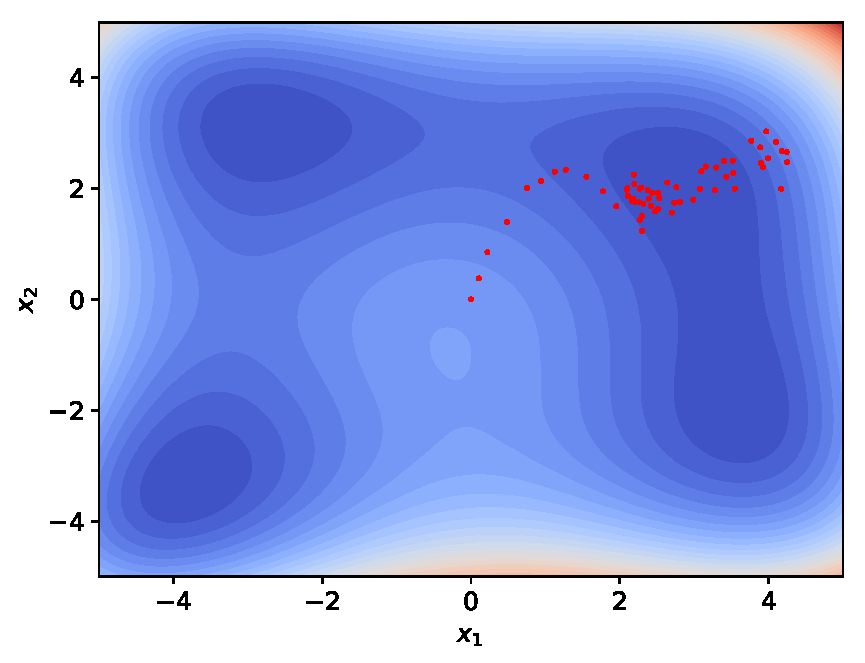
\includegraphics[width=\textwidth]{graphics/var-opt-conv/VO-R-himmelblau-convergence.pdf}
            \caption{}
            \label{fig: Theory: var-opt-conv-VO-R-himmelblau-convergence}
        \end{subfigure}
        \hfill
        \begin{subfigure}[b]{0.49\textwidth}
            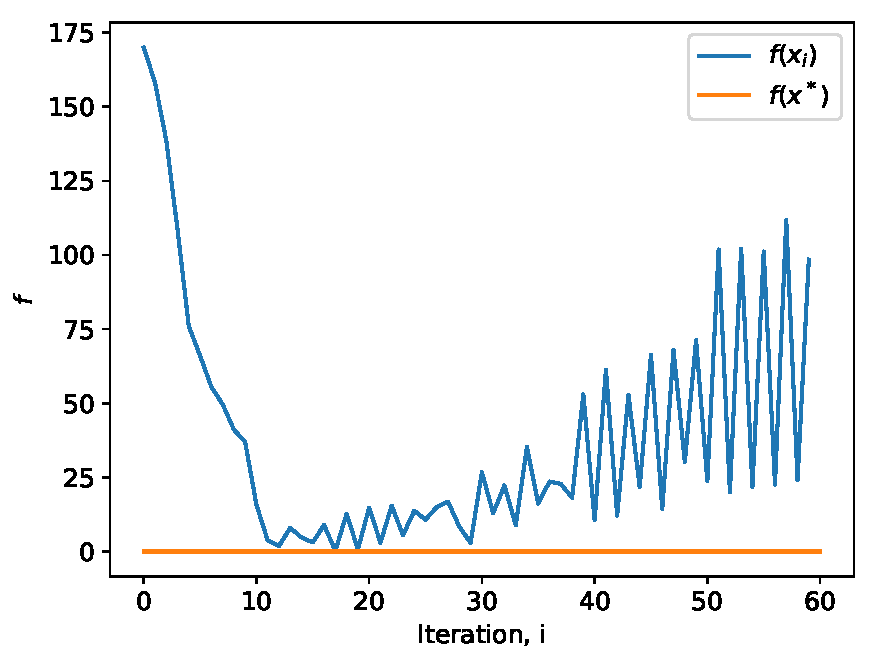
\includegraphics[width=\textwidth]{graphics/var-opt-conv/VO-R-himmelblau-f.pdf}
            \caption{}
            \label{fig: Theory: var-opt-conv-VO-R-himmelblau-f}
        \end{subfigure}
        \caption{\subref{fig: Theory: var-opt-conv-VO-R-himmelblau-convergence} Convergence of the \gls{VO} algorithm with isotropic Gaussian search distribution using regular gradients. \subref{fig: Theory: var-opt-conv-VO-R-himmelblau-f} Objective function value at each iteration. Similarly to fixed variance \gls{ES}, a minimum is found, but the optimization of the variance drives it towards zero, resulting in larger gradients and variance.}
        \label{fig: Theory: var-opt-conv-VO-R-himmelblau}
    \end{figure}
}


\section{Natural gradient}

\subsection{Search space distance}

\frame{
    \frametitle{Motivation}
    \begin{block}{Problems with regular search gradients}
        \tabitem \textbf{Cannot precisely locate any optimum} since gradient explodes for $\sigma\rightarrow0$.\\
        \tabitem Want to make small change to search distribution parameters
        \begin{equation}
            p(\w|\thetab) \leftarrow p(\w|\thetab+\Delta\thetab)
        \end{equation}
        but regular gradient defines distance in Euclidean terms, $\sqrt{\Delta\thetab\transpose\Delta\thetab}$, which is dependent on search distribution parameterization and inappropriate in high dimensions.\\
        \tabitem Is it possible to obtain a gradient that is invariant to parameterization, i.e. \textbf{do gradient descent with respect to an invariant measure of the closeness of the current distribution and the updated distribution}?
    \end{block}
}

\frame{
    \frametitle{Distance measure}
    \begin{block}{\gls{KL}}
        \tabitem Measures distance between \glspl{PDF} \cite{Kullback1951}\\
        \begin{equation}
            \begin{aligned}
                \text{KL}\pa{p||q} &\equiv -\int p(\w)\log q(\w) \;\text{d}\w + \int p(\w)\log p(\w) \;\text{d}\w\\
                &= -\int p(\w)\log\pa{\frac{q(\w)}{p(\w)}}\;\text{d}\w
            \end{aligned}
        \end{equation}
        \tabitem It can be symmetrized and approximated by Taylor series
        \begin{equation}
            \text{KL}\pa{p(\w|\thetab) , p(\w|\thetab+\Delta\thetab)} \approx \frac{1}{2}\Delta\thetab\transpose\F_\thetab\Delta\thetab
        \end{equation}
    \end{block}
    \begin{block}{Fisher information matrix}
        \begin{equation}
            \F_\thetab \equiv \text{E}\bra{\nabla_\thetab\log p(\w|\thetab)\nabla_\thetab\log p(\w|\thetab)\transpose}
        \end{equation}
        % \begin{align}
        %     \F_\thetab &\equiv \text{E}\bra{\nabla_\thetab\log p(\w|\thetab)\nabla_\thetab\log p(\w|\thetab)\transpose}\\
        %     &= \text{Cov}\bra{\nabla_\thetab\log p(\w|\thetab)}\\
        %     &= -\text{E}\bra{\nabla_\thetab^2\log p(\w|\thetab)}
        % \end{align}
    \end{block}
}

\subsection{Steepest descent w.r.t. a distance metric}

\frame{
    \frametitle{Steepest descent w.r.t. a distance metric}
    \begin{block}{Fixing the per iteration search distribution change}
        \tabitem Each minimization step $\Delta\thetab$ on the variational upper bound $U(\thetab)$ can be written as a Taylor expansion
        \begin{equation}
            U(\thetab + \Delta\thetab) \approx U(\thetab) + \Delta\thetab\transpose\nabla_\thetab U(\thetab)
        \end{equation}
        \tabitem The search gradient can then be found by minimizing the variational upper bound while keeping the \gls{KL} divergence fixed to a small constant, $\kappa$.
        \begin{equation}
            \begin{aligned}
                &\min_\thetab U(\thetab + \Delta\thetab) \approx U(\thetab) + \Delta\thetab\transpose\nabla_\thetab U(\thetab)\\
                & \text{s.t. } \text{KL}\pa{p(\w|\thetab) , p(\w|\thetab+\Delta\thetab)} \approx \frac{1}{2}\Delta\thetab\transpose\F_\thetab\Delta\thetab = \kappa
            \end{aligned}
        \end{equation}
        \tabitem This has the so-called natural gradient as solution (search direction)
        \begin{equation}
            \tilde{\nabla}_\thetab U(\thetab) = \alpha\F_\thetab^{-1}\nabla_\thetab U(\thetab)
        \end{equation}
    \end{block}
}


\frame{
    \begin{block}{Natural gradient for univariate Gaussian}
        \tabitem Fischer information matrix can be found analytically
        \begin{equation}
            \F_\thetab = \bmat{\frac{1}{\sigma^2} & 0\\
                                0 & \frac{1}{2\sigma^4}}\quad\Longleftrightarrow\quad 
            \F_\thetab^{-1} = \bmat{\sigma^2 & 0\\
                                0 & 2\sigma^4}
        \end{equation}
        \tabitem The gradient is scaled by $\F_\thetab^{-1}$
        \begin{equation}
            \begin{aligned}
                \sigma^2\pderiv{}{\mu}U(\mu,\sigma^2) &= \sigma\text{E}\bra{f(\mu + \sigma\epsilon)\epsilon} \approx \frac{\sigma}{N}\sum_{n=1}^N f(\mu+\sigma\epsilon_n)\epsilon_n\\
                2\sigma^4\pderiv{}{\sigma^2}U(\mu,\sigma^2) &= \text{E}\bra{f(\mu + \sigma^2\sigma\epsilon)\left(\epsilon^2-1\right)} \approx \frac{\sigma^2}{N}\sum_{n=1}^N f(\mu + \sigma\epsilon_n)\left(\epsilon_n^2-1\right)\\
            \end{aligned}\label{eq: Theory: Variational optimization univariate gaussian gradient estimators natural gradient}
        \end{equation}
        \tabitem This can be done similarly for the isotropic and separable Gaussians
    \end{block}
}

\frame{
    \frametitle{Himmelblau example 3}
    \begin{figure}[tbp!]
        \begin{subfigure}[b]{0.49\textwidth}
            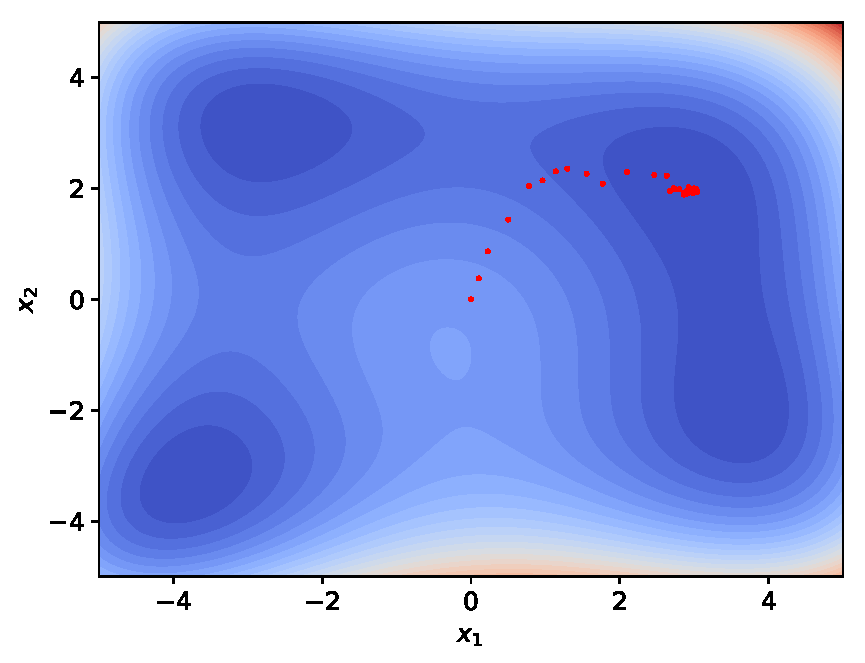
\includegraphics[width=\textwidth]{graphics/var-opt-conv/VO-N-himmelblau-convergence.pdf}
            \caption{}
            \label{fig: Theory: var-opt-conv-VO-N-himmelblau-convergence}
        \end{subfigure}
        \hfill
        \begin{subfigure}[b]{0.49\textwidth}
            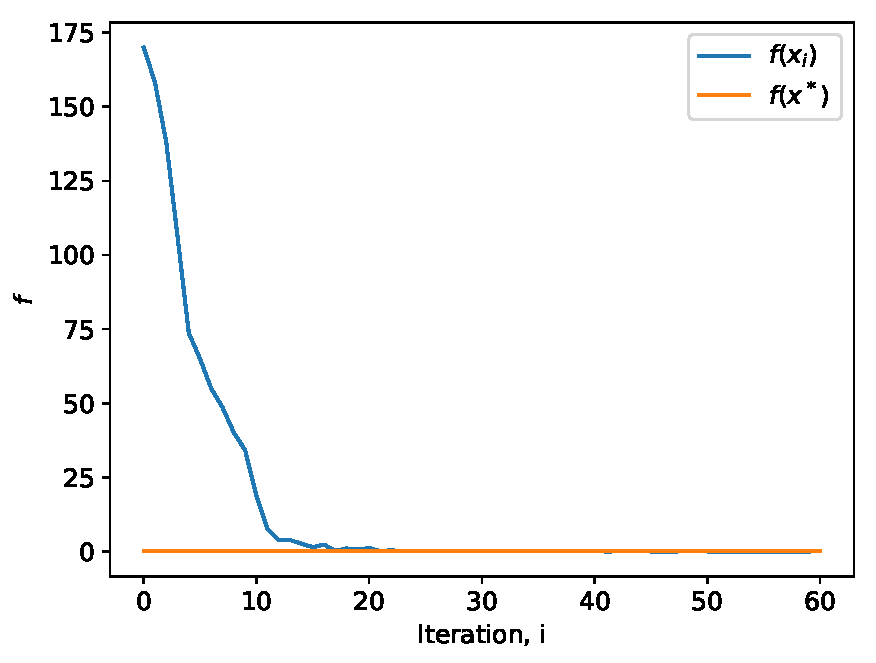
\includegraphics[width=\textwidth]{graphics/var-opt-conv/VO-N-himmelblau-f.pdf}
            \caption{}
            \label{fig: Theory: var-opt-conv-VO-N-himmelblau-f}
        \end{subfigure}
        \caption{\subref{fig: Theory: var-opt-conv-VO-N-himmelblau-convergence} Convergence of the variational optimization algorithm with isotropic Gaussian search distribution using natural gradients. \subref{fig: Theory: var-opt-conv-VO-N-himmelblau-f} Objective function value at each iteration. A minimum is found and the optimization of the variance drives the gradients toward zero resulting in convergence to the optimum.}
        \label{fig: Theory: var-opt-conv-VO-N-himmelblau}
    \end{figure}
}


\section{Variance reduction}

\subsection{Antithetic sampling}

\frame{
    \frametitle{Antithetic sampling}
    \begin{block}{Shorthand notation and odd/even decomposition}
        \tabitem Let $g(\w) = f(\w) \nabla_\thetab\log p(\w|\thetab)$ so $\nabla_\thetab U(\thetab) = \frac{1}{N}\sum_{n=1}^N g(\w)$\\
        \tabitem Any function $g(\w) = g_e(\w) + g_o(\w)$ where $g_e$ and $g_o$ are even and odd parts
    \end{block}
    
    \begin{block}{Leveraging covariance between perturbations}
    \tabitem Rather than sampling $\epsilonb_n$ IID, take every other to be $-\epsilonb_i$ and decompose $g$
    \begin{equation}
        \nabla_\thetab U_a(\thetab) = \frac{1}{N}\sum_{n=1}^{N/2} g(\w_n) + g(-\w_n) = \frac{2}{N}\sum_{n=1}^{N/2} g_e(\w_i)
    \end{equation}
    \tabitem Due to this trick, there is again zero covariance and the variance simplifies 
    \begin{equation}
        \text{Var}\bra{\nabla_\thetab U_a(\thetab)} = \frac{2}{N}\text{Var}\bra{g_e(\w)}
    \end{equation}
    
    
    % \begin{equation}
    %     \nabla_\thetab U(\thetab) = \frac{1}{N}\sum_{n=1}^N g(\w_i) = \frac{2}{N}\sum_{n=1}^{N/2} g_e(\w_i)
    % \end{equation}
    
    \tabitem Compared to the IID sampling result \eqref{eq: Gradient variance: ES Isoptropic Gaussian in terms of f and eps}, antithetic sampling trades in the variance of $g$ for two times the variance of $g_e$.\\
    \tabitem If $g_e$ is zero everywhere then $\text{Var}\bra{\nabla_\thetab U_a(\thetab)}=0$\\
    \tabitem If $g_o$ is zero everywhere then $\text{Var}\bra{\nabla_\thetab U_a(\thetab)}=2\text{Var}\bra{\nabla_\thetab U(\thetab)}$
    
    % \begin{equation}
    %     \text{Var}\bra{\nabla_\thetab U(\thetab)} = \text{Var}\bra{\frac{1}{N}\sum_{n=1}^N g(\w_i)} = \frac{1}{N}\text{Var}\bra{g(\w)} + \frac{2}{N^2}\sum_{i=1}^N\sum_{j=i+1}^N\text{Cov}\bra{g(\w_i), g(\w_j)}\label{eq: Theory: Variance of multivariate Gaussian variational optimization gradient estimator regular samplng}
    % \end{equation}
    %     \begin{equation}
    %         \text{Var}\left[\nabla_\w f(\w)\right]
    %         \approx \text{Var}\left[\frac{1}{N\sigma}\sum_{n=1}^N f(\w+\sigma\epsilonb_n)\epsilonb_n\right]
    %         = \frac{1}{N\sigma^2}\text{Var}\bra{f(\w+\sigma\epsilonb)\epsilonb} \ . 
    %     \end{equation}
    \end{block}
}

\frame{
    \frametitle{Results for antithetic sampling}
    \begin{figure}[tbp!]
        \begin{subfigure}[b]{0.49\textwidth}
            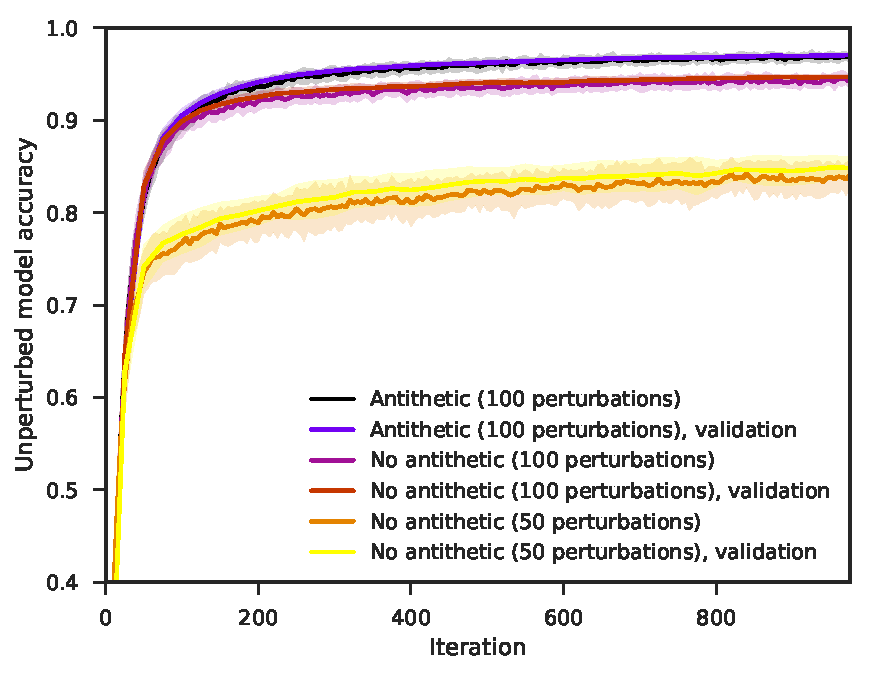
\includegraphics[width=\textwidth]{graphics/E022-AS-analysis/accuracy_unp-all-series-mean-sd.pdf}
            \caption{}
            \label{fig: Theory: E022-AS-analysis/accuracy_unp-all-series-mean-sd}
        \end{subfigure}
        \hfill
        \begin{subfigure}[b]{0.49\textwidth}
            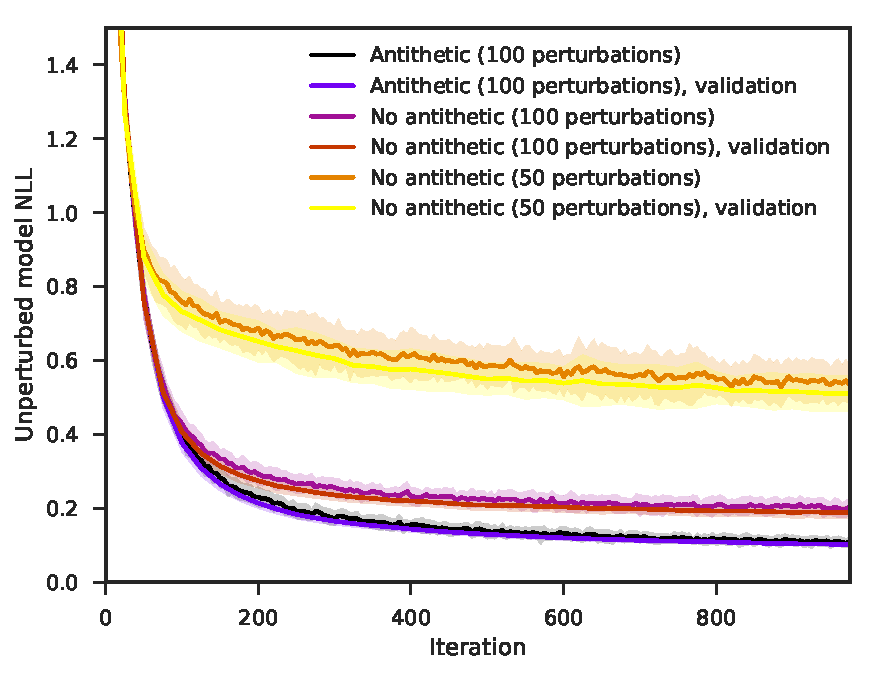
\includegraphics[width=\textwidth]{graphics/E022-AS-analysis/return_unp-all-series-mean-sd.pdf}
            \caption{}
            \label{fig: Theory: E022-AS-analysis/return_unp-all-series-mean-sd}
        \end{subfigure}
        \caption{
            Results of training a neural network with \gls{VO} and antithetic sampling on handwritten digit recognition.
            \subref{fig: Theory: E022-AS-analysis/accuracy_unp-all-series-mean-sd} Training and validation set classification accuracy.
            \subref{fig: Theory: E022-AS-analysis/return_unp-all-series-mean-sd} Training and validation set \gls{NLL} loss.
        }
        \label{fig: Theory: E022-AS-analysis}
    \end{figure}
}

\subsection{Local reparameterization}

\frame{
    \frametitle{Local reparameterization}
    \begin{block}{Introducing the mini-batch}
        \tabitem When the objective/error is a sum of individual terms from a mini-batch $\mathcal{B}$
        \begin{equation}
            U(\thetab) \approx \frac{1}{N\size{\mathcal{B}}}\sum_{n=1}^N\sum_{b\in\mathcal{B}} f_b(\w_n)
        \end{equation}
        \tabitem This introduces covariance between batch examples (despite IID perturbations)
        \begin{equation}
            \text{Var}\bra{U(\thetab)} \approx \frac{1}{N\size{\mathcal{B}}}\text{Var}\bra{f_b(\w)} + \frac{N-1}{N}\frac{\size{\mathcal{B}}-1}{\size{\mathcal{B}}}\text{Cov}\bra{f_b(\w),f_{b'}(\w)}
        \end{equation}
    \end{block}
    \begin{block}{Removing within-batch covariance}
        \tabitem By sampling new weights for each batch example, $\w_b$, this covariance vanishes \cite{Kingma2015a}
        \begin{equation}
            \text{Var}\bra{\tilde{U}(\thetab)} \approx \frac{1}{N\size{\mathcal{B}}}\text{Var}\bra{f_b(\w_b)}
        \end{equation}
    \end{block}
}

\frame{
    \frametitle{Local reparameterization}
    \begin{block}{Upper bound gradient}
        \tabitem The gradient is similar to before but now summed over the mini-batch as well
        \begin{equation}
            \nabla_\thetab \tilde{U}(\thetab) \approx \frac{1}{N\size{\mathcal{B}}}\sum_{n=1}^N\sum_{b\in\mathcal{B}}f_b(\w_{bn})\nabla_\thetab\log p(\w_{bn}|\thetab)
        \end{equation}
        \tabitem Computationally inefficient due to new weights for each batch example\\
        % \tabitem Here: Many networks, one example, $N$ times\\
        % \tabitem Libraries: One network, many examples, once
    \end{block}
    \begin{block}{Propagating a distribution over activations}
        % \tabitem In \gls{FNN}, $\Z^\bra{l}=\W^\bra{l}\A^\bra{l-1}$ where $\A^\bra{l}=\varphi\pa{\Z^\bra{l}}$\\
        % \tabitem Take an isotropic Gaussian search distribution $p(\W|\thetab)=\mathcal{N}\pa{\W|\mub,\sigma^2\I}$\\
        \tabitem Can infer distribution of activations from distribution of weights in \gls{FNN}\\
        \begin{equation}
            q\pa{Z_{ib}^\bra{l} \;\middle|\; \A^\bra{l-1}, \thetab} = \mathcal{N}\left(Z_{ib}^\bra{l} \;\middle|\; \sum_j \mu_{ij}^\bra{l} A_{jb}^\bra{l-1}, \sum_j \sigma^{\bra{l}^2}_{ij} A^{\bra{l-1}^2}_{jb}\right)
            %= \mathcal{N}\left(Z_{ib}^\bra{l} \;\middle|\; m_{ib}^\bra{l}, v_{ib}^\bra{l}\right)
        \end{equation}
        \tabitem Here, $\Z^\bra{l}=\W^\bra{l}\A^\bra{l-1}$, $\A^\bra{l}=\varphi\pa{\Z^\bra{l}}$ and $p(\W|\thetab)=\mathcal{N}\pa{\W|\mub,\sigma^2\I}$
    \end{block}
    
}

\frame{
    \frametitle{Local reparameterization}
    \begin{block}{New gradient}
        \tabitem Gradient is then obtained by perturbing the activation space
        \begin{equation}
            \nabla_\thetab \tilde{U}(\theta) \approx \frac{1}{N\size{\mathcal{B}}} \sum_{n=1}^N\sum_{b\in\mathcal{B}} f_b(\Z_{bn}) \nabla_\thetab
            \log q(\Z_{bn}|\A_{bn},\thetab)
        \end{equation}
    \end{block}
    \begin{block}{Gradient in \gls{FNN}}
        \tabitem Specifically, for an \gls{FNN}\\
        \begin{equation}\label{eq: Theory: Local reparameterization: Gradient of upper bound isotropic/full Gaussian}
            \begin{aligned}
                \pderiv{\tilde{U}(\thetab)}{\mu_{ij}^\bra{l}} &\approx \frac{1}{N\size{\mathcal{B}}} \sum_{n=1}^N\sum_ {b\in\mathcal{B}} f_b(\Z_{bn}) \frac{\xi_{ibn}}{\sqrt{v_{ib}^\bra{l}}} A_{jb}^\bra{l-1} \\
                \pderiv{\tilde{U}(\thetab)}{\sigma_{ij}^{\bra{l}^2}} &\approx \frac{1}{N\size{\mathcal{B}}} \sum_{n=1}^N\sum_ {b\in\mathcal{B}} f_b(\Z_{bn}) \frac{\xi_{ibn}^2 - 1}{2 v_{ib}^\bra{l}} A_{jb}^{\bra{l-1}^2} \ .
                %\frac{dU(\theta)}{d\mu_{ij}} &\approx \frac{1}{N} \sum_{n=1}^N\sum_ {b\in\mathcal{B}} \widehat{F}_m(Z_{bn}) \frac{\xi_{ims}}{\sqrt{v_{im}}} A_{jm} \\ 
                %\frac{dU(\theta)}{d\sigma_{ij}^2} & \approx \frac{1}{N} \sum_{n=1}^N\sum_ {b\in\mathcal{B}} \widehat{F}_m(Z_{bn}) \frac{\xi_{ims}^2 - 1}{2 v_{im}} A_{jm}^2 \ .
            \end{aligned}
        \end{equation}
        where $Z_{ibn} = m_{ib} + \sqrt{v_{ib}}\,\xi_{ibn}$, with $\xi_{ibn}\sim\mathcal{N}(0,1)$
    \end{block}
}

\frame{
    \frametitle{Local reparameterization}
    \begin{block}{Forward pass in \gls{FNN}}
        \tabitem With $\A^\bra{0} = \X$ as a batch of inputs, the forward pass in an \gls{FNN} is
        \begin{subequations}
            \begin{align}
                \m^\bra{l} & = \mub^\bra{l} \A^\bra{l-1} \\
                \v^\bra{l} & = \left( \sigmab^\bra{l} \A^\bra{l-1}\right)^2 \\
                \Z^\bra{l} & = \m^\bra{l} + \sqrt{\v^\bra{l}} \odot \xib^\bra{l}\\
                \A^\bra{l} &= \varphi\pa{\Z^\bra{l}}
            \end{align}
        \end{subequations}
        \tabitem Forward propagation of a distribution over activations
    \end{block}
    
    %The complexity of a forward pass with this new approach is $\mathcal{O}\pa{N\size{\mathcal{B}}\size{\Z}}$ where $\size{\Z}$ is the number of activations/units in the network. The batch can be efficiently forward propagated in a single pass as described in \autoref{chp: Neural networks}. For comparison, the original approach has a complexity of $\mathcal{O}\pa{N\size{\W}}$ while a naive implementation of local reparameterization has a complexity of $\mathcal{O}\pa{N\size{\mathcal{B}}\size{\W}}$ and additionally requires a forward pass for each batch example which is less efficient than the new approach. The local reparameterization thus improves computational efficiency by sampling activations rather than weights.
    
   % With $\A^\bra{0} = \X$, the forward pass in an \gls{FNN} then %$Z^\bra{l}_{ib} = m^{(l)}_{ib} + \sqrt{v^{(l)}_{ib}} \xi^{(l)}_{ib}$ or 
}

\section*{Conclusion}


\frame{
    \frametitle{Conclusion}
    
    \begin{block}{Conclusion}
        \tabitem Variational optimization\\
        \tabitem Natural gradient\\
        \tabitem Variance reduction\\
    \end{block}
    
    \begin{block}{Other topics}
        \tabitem Adapting the variance\\
        \tabitem Sensitivity rescaled perturbations\\
        \tabitem Reuse of samples (importance mixing)\\
        \tabitem Adapting hyperparameters by adaptation sampling\\
        \tabitem Fitness transforms\\
    \end{block}
    
    \begin{block}{Future work}
        \tabitem How does local reparameterization fare in practice?\\
        \tabitem Is there a way around the problems with adapting the variance? Separable Gaussian did not harm performance\\
        \tabitem How to compute importance weights in high dimensional spaces in order to use importance mixing and adaptation sampling?\\
    \end{block}
    
    % \begin{block}{Weight space VS activation space}
    %     \tabitem Is direct optimization in weight space necessary?\\
    %     \tabitem Since perturbations are normal, this provides a way to propagate perturbation distribution to activations.\\
    %     \tabitem One could perturb the activations and map these to weight gradients, shrinking the effective search space for fully connected linear layers \cite{Kingma2015a}.\\
    % \end{block}
}

